% Author: Izaak Neutelings (October 2020)
\documentclass[border=3pt,tikz]{standalone}
\usepackage{physics}
\usepackage{tikz}
\usepackage[outline]{contour} % glow around text
\usetikzlibrary{calc}
\usetikzlibrary{angles,quotes} % for pic
\usetikzlibrary{arrows.meta}
\usetikzlibrary{patterns}
\tikzset{>=latex} % for LaTeX arrow head
\contourlength{1.35pt}

\colorlet{xcol}{blue!70!black}
\colorlet{vcol}{green!60!black}
\colorlet{myred}{red!65!black}
\colorlet{mypurple}{blue!60!red!80}
\colorlet{acol}{red!50!blue!80!black!80}
\tikzstyle{rvec}=[->,xcol,very thick,line cap=round]
\tikzstyle{vvec}=[->,vcol,very thick,line cap=round]
\tikzstyle{myarr}=[{Latex[length=3,width=3]}-,xcol]
\tikzstyle{myarr2}=[{Latex[length=2,width=3]}-{Latex[length=2,width=3]}]
\tikzstyle{force}=[->,myred,very thick,line cap=round]
\tikzstyle{Fproj}=[force,myred!40]
\tikzstyle{CM}=[draw=red!40!black,fill=red!80!black!80]
\tikzstyle{mass}=[line width=0.6,draw=red!30!black, %rounded corners=1,
                  top color=red!40!black!30,bottom color=red!40!black!10,shading angle=30]
\tikzstyle{ground}=[preaction={fill,top color=black!10,bottom color=black!5,shading angle=20},
                    fill,pattern=north east lines,draw=none,minimum width=0.3,minimum height=0.6]
\tikzstyle{metal}=[fill,top color=black!40,bottom color=black!20,shading angle=10]


\def\r{0.05} % pulley small radius
\tikzset{
  pics/Tin/.style={
    code={
      \def\R{0.12}
      \draw[pic actions,line width=0.6,#1,fill=white] % ,thick
        (0,0) circle (\R) (-135:.75*\R) -- (45:.75*\R) (-45:.75*\R) -- (135:.75*\R);
  }},
  pics/Tout/.style={
    code={
      \def\R{0.12}
      \draw[pic actions,line width=0.6,#1,fill=white] (0,0) circle (\R);
      \fill[pic actions,#1] (0,0) circle (0.3*\R);
  }},
  pics/rotarr/.style={
    code={
      \draw[white,very thick] ({#1*cos(200)},0) arc(-200:30:{#1} and {#1/2}) --++ (125:0.1);
      \draw[->] ({#1*cos(200)},0) coordinate (W1) arc(-200:20:{#1} and {#1/2}) node[midway] (W2) {} --++ (125:0.1) coordinate (W3);
  }},
  pics/Tin/.default=mypurple,
  pics/Tout/.default=mypurple,
  pics/rotarr/.default=0.4,
}

\begin{document}


% DISK - no angular momentum
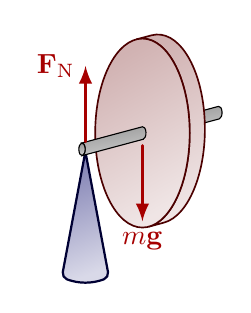
\begin{tikzpicture}
  \def\h{1.6}  % pivot height
  \def\w{0.6}  % pivot width
  \def\t{0.2}  % wheel thickness
  \def\R{1.2}  % wheel radius
  \def\b{0.5}  % wheel radius horizontal scale
  \def\L{0.8}  % handle length
  \def\r{0.08} % handle radius
  \def\ang{15}
  \coordinate (O) at (0,0);
  \coordinate (T) at (-40:1.8*\t);
  \coordinate (F) at (-\L+0.05,0);
  \draw[thick,rounded corners=2,blue!20!black,
        top color=blue!40!black!50,bottom color=blue!40!black!15,shading angle=20]
    (\ang-180:\L-0.05)++(0,-\r+0.04) --++ (-\w/2,-\h) to[out=-20,in=-160]++ (\w,0) -- cycle;
  \draw[metal]
    (\ang:\t)++(0,\r)
      arc(90+\ang/2:-90+\ang/2:{\r*\b} and \r) --++ (\ang:\L) coordinate (P)
      arc(-90+\ang/2:90+\ang/2:{\r*\b} and \r) -- cycle;
  \draw[mass]
    (90+\ang/2:{\b*\R} and \R) --++ (\ang:\t)
    arc(90+\ang/2:-90+\ang/2:{\b*\R} and \R) --++ (\ang-180:\t)
    arc(-90+\ang/2:90+\ang/2:{\b*\R} and \R);
  \draw[mass,rounded corners=0.9] (O) ellipse ({\b*\R} and \R);
  \draw[metal]
    (0,\r) arc(90+\ang/2:-90+\ang/2:{\r*\b} and \r) --++ (\ang-180:\L) coordinate (P)
           arc(-90+\ang/2:90+\ang/2:{\r*\b} and \r) coordinate (F) -- cycle;
  \draw[metal] (P) arc(-90+\ang/2:270+\ang/2:{\r*\b} and \r);
  \draw[force] (F)++(0.05,0.02) --++ (0,0.8*\R) node[left=0] {$\vb{F}_\mathrm{N}$};
  \draw[force] (O)++(0,-2*\r) --++ (0,-0.8*\R) node[below=0] {$m\vb{g}$};
\end{tikzpicture}



% DISK - no angular momentum
\def\h{1.6}  % pivot height
\def\w{0.6}  % pivot width
\def\t{0.2}  % wheel thickness
\def\R{1.2}  % wheel radius
\def\L{0.8}  % handle length
\def\r{0.06} % handle radius
\begin{tikzpicture}
  \coordinate (O) at (0,0);
  \coordinate (T) at (-40:1.8*\t);
  \coordinate (P) at (-\L+0.05,-0.02);
  \coordinate (F) at (-\L+0.05,0);
  \draw[ground] (-1.7*\L,-\h-0.02) rectangle++ (3.2*\L,-\t);
  \draw[thick] (-1.7*\L,-\h-0.02) --++ (3.2*\L,0);
  \draw[thick,rounded corners=2,blue!20!black,
        top color=blue!40!black!50,bottom color=blue!40!black!15,shading angle=20]
    (P) --++ (-\w/2,-\h) --++ (\w,0) -- cycle; %++(0,0.02)
  \draw[metal] (O)++(-\L,-\r) rectangle++ (2*\L,2*\r);
  \draw[mass,rounded corners=0.9] (O)++(-\t/2,-\R) rectangle++ (\t,2*\R);
  \draw[dashed,xcol] (F)++(60:\L-0.05) arc(60:-60:\L-0.05);
  \draw[->] (F)++(42:1.9*\L) arc(70:0:0.5*\L) node[midway,above right=-2] {$\alpha$};
  \draw[CM] (O) circle(0.35*\t); %node[above right=2,scale=0.9] {$M$};
  \draw[rvec] (F) -- (O) node[midway,above] {$\vb{r}$};
  \draw[force] (O) --++ (0,-0.8*\R) node[right=1] {$M\vb{g}$};
  \draw[force] (F) --++ (0,0.8*\R) node[left=0] {$\vb{F}_\mathrm{N}$};
  \pic[scale=1] at (T) {Tin};
  \node[mypurple,below=2,right=1] at (T) {$\vb*\tau$};
  \node[vcol,right,scale=0.8] at (60:2.0*\t) {$\vb{L}=0$};
\end{tikzpicture}


% DISK - angular momentum
\begin{tikzpicture}
  \coordinate (O) at (0,0);
  \coordinate (T) at (-40:1.8*\t);
  \coordinate (P) at (-\L+0.05,-0.02);
  \coordinate (F) at (-\L+0.05,0);
  \draw[ground] (-1.7*\L,-\h-0.02) rectangle++ (3.2*\L,-\t);
  \draw[thick] (-1.7*\L,-\h-0.02) --++ (3.2*\L,0);
  \draw[thick,rounded corners=2,blue!20!black,
        top color=blue!40!black!50,bottom color=blue!40!black!15,shading angle=20]
    (P) --++ (-\w/2,-\h) --++ (\w,0) -- cycle; %++(0,0.02)
  \draw[metal] (O)++(-\L,-\r) rectangle++ (2*\L,2*\r);
  \draw[mass,rounded corners=0.9] (O)++(-\t/2,-\R) rectangle++ (\t,2*\R);
  \draw[force,vcol]
    (O) --++ (1.9*\L,0) node[right=-1] {$\vb{L}$};
  \draw[CM] (O) circle(0.35*\t); %node[above right=2,scale=0.9] {$M$};
  \draw[rvec] (F) -- (O) node[midway,above] {$\vb{r}$};
  \draw[force] (O) --++ (0,-0.8*\R) node[right=1] {$M\vb{g}$};
  \draw[force] (F) --++ (0,0.8*\R) node[left=0] {$\vb{F}_\mathrm{N}$};
  \pic[scale=1] at (T) {Tin};
  \node[mypurple,below=2,right=1] at (T) {$\vb*\tau$};
\end{tikzpicture}


% DISK - angular momentum - top view
\begin{tikzpicture}
  \coordinate (O) at (0,0);
  %\coordinate (T) at (-40:1.8*\t);
  \coordinate (F) at (-\L+0.05,0);
  \coordinate (L) at (1.9*\L,0);
  \draw[thick,rounded corners=2,blue!20!black,
        top color=blue!40!black!50,bottom color=blue!40!black!15,shading angle=20]
    (F) circle(\w/2);
  \draw[metal] (O)++(-\L,-\r) rectangle++ (2*\L,2*\r);
  \draw[mass,rounded corners=0.9] (O)++(-\t/2,-\R) rectangle++ (\t,2*\R);
  \draw[CM] (O) circle(0.35*\t); %node[above right=2,scale=0.9] {$M$};
  \draw[dashed,xcol] (F) circle(\L-0.05);
  \draw[force,vcol!80!black!50] (O) --++ (20:1.9*\L) coordinate (DL); 
  \draw[force,vcol!80!black!50] (L) -- (DL) node[right=-1] {$\dd{\vb{L}}$};
  \draw[force,vcol] (O) -- (L) node[below=-1] {$\vb{L}$};
  \draw[force,acol] (O) --++ (0,0.7*\R) node[below right=1] {$\vb*{\tau}$};
  %\pic[scale=1] at (T) {Tin};
  %\node[mypurple,below=2,right=1] at (T) {$\vb*\tau$};
  \draw[->] (F)++(110:1.3*\L) arc(110:160:1*\L) node[midway,above left=-3] {$\omega_\mathrm{p}$};
  \draw pic["$\dd{\theta}$",draw,angle radius=24.5,angle eccentricity=1.28] {angle=L--O--DL};
\end{tikzpicture}


% DISK - angular momentum
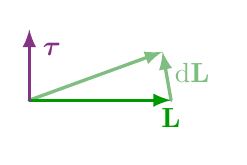
\begin{tikzpicture}
  \def\L{1.8}
  \coordinate (O) at (0,0);
  \coordinate (L) at (\L,0);
  \draw[force,vcol!80!black!50] (O) --++ (20:\L) coordinate (DL); 
  \draw[force,vcol!80!black!50] (L) -- (DL) node[midway,above=1,right=-1] {$\dd{\vb{L}}$};
  \draw[force,vcol] (O) -- (L) node[below=-1] {$\vb{L}$};
  \draw[force,acol] (O) --++ (0,0.5*\L) node[below right=1] {$\vb*{\tau}$};
  %\draw[dashed,xcol] (F) circle(\L-0.05);
\end{tikzpicture}



\end{document}
